


\documentclass[a0paper,portrait]{baposter}\usepackage[]{graphicx}\usepackage[]{color}
%% maxwidth is the original width if it is less than linewidth
%% otherwise use linewidth (to make sure the graphics do not exceed the margin)
\makeatletter
\def\maxwidth{ %
  \ifdim\Gin@nat@width>\linewidth
    \linewidth
  \else
    \Gin@nat@width
  \fi
}
\makeatother

\definecolor{fgcolor}{rgb}{0.345, 0.345, 0.345}
\newcommand{\hlnum}[1]{\textcolor[rgb]{0.686,0.059,0.569}{#1}}%
\newcommand{\hlstr}[1]{\textcolor[rgb]{0.192,0.494,0.8}{#1}}%
\newcommand{\hlcom}[1]{\textcolor[rgb]{0.678,0.584,0.686}{\textit{#1}}}%
\newcommand{\hlopt}[1]{\textcolor[rgb]{0,0,0}{#1}}%
\newcommand{\hlstd}[1]{\textcolor[rgb]{0.345,0.345,0.345}{#1}}%
\newcommand{\hlkwa}[1]{\textcolor[rgb]{0.161,0.373,0.58}{\textbf{#1}}}%
\newcommand{\hlkwb}[1]{\textcolor[rgb]{0.69,0.353,0.396}{#1}}%
\newcommand{\hlkwc}[1]{\textcolor[rgb]{0.333,0.667,0.333}{#1}}%
\newcommand{\hlkwd}[1]{\textcolor[rgb]{0.737,0.353,0.396}{\textbf{#1}}}%

\usepackage{framed}
\makeatletter
\newenvironment{kframe}{%
 \def\at@end@of@kframe{}%
 \ifinner\ifhmode%
  \def\at@end@of@kframe{\end{minipage}}%
  \begin{minipage}{\columnwidth}%
 \fi\fi%
 \def\FrameCommand##1{\hskip\@totalleftmargin \hskip-\fboxsep
 \colorbox{shadecolor}{##1}\hskip-\fboxsep
     % There is no \\@totalrightmargin, so:
     \hskip-\linewidth \hskip-\@totalleftmargin \hskip\columnwidth}%
 \MakeFramed {\advance\hsize-\width
   \@totalleftmargin\z@ \linewidth\hsize
   \@setminipage}}%
 {\par\unskip\endMakeFramed%
 \at@end@of@kframe}
\makeatother

\definecolor{shadecolor}{rgb}{.97, .97, .97}
\definecolor{messagecolor}{rgb}{0, 0, 0}
\definecolor{warningcolor}{rgb}{1, 0, 1}
\definecolor{errorcolor}{rgb}{1, 0, 0}
\newenvironment{knitrout}{}{} % an empty environment to be redefined in TeX

\usepackage{alltt}

\usepackage{relsize}		% For \smaller
\usepackage{url}			% For \url
\usepackage{epstopdf}	% Included EPS files automatically converted to PDF to include with pdflatex
\usepackage{amsmath}
\usepackage{amssymb}
\usepackage{array}
\usepackage{tabularx}
\usepackage{booktabs}
\DeclareMathOperator*{\argmax}{arg\,max}
\newcommand{\bi}{\begin{itemize}}
\newcommand{\ei}{\end{itemize}}
\newcommand{\tr}{\textit{true}}
\newcommand{\true}{\textit{true}}
\newcommand{\naive}{\textit{recent}}
\newcommand{\recent}{\textit{recent}}
\newcommand{\default}{\textit{all-time}}
\newcommand{\market}{\textit{market}}
\newcommand{\Market}{\textit{Market}}
\newcommand{\raw}{\texttt{last}}
\newcommand{\last}{\texttt{last}}
\newcommand{\diff}{\texttt{diff}}
\newcommand{\random}{\texttt{random}}
\newcommand{\rollsd}{\texttt{roll.sd}}
%%% Global Settings %%%%%%%%%%%%%%%%%%%%%%%%%%%%%%%%%%%%%%%%%%%%%%%%%%%%%%%%%%%

%\graphicspath{{pix/}}	% Root directory of the pictures
\tracingstats=2			% Enabled LaTeX logging with conditionals

%%% Color Definitions %%%%%%%%%%%%%%%%%%%%%%%%%%%%%%%%%%%%%%%%%%%%%%%%%%%%%%%%%

\definecolor{bordercol}{RGB}{40,40,40}
\definecolor{headercol1}{RGB}{186,215,230}
\definecolor{headercol2}{RGB}{80,80,80}
\definecolor{headerfontcol}{RGB}{0,0,0}
%\definecolor{boxcolor}{RGB}{186,215,230}
\definecolor{boxcolor}{RGB}{224,255,255}
%%%%%%%%%%%%%%%%%%%%%%%%%%%%%%%%%%%%%%%%%%%%%%%%%%%%%%%%%%%%%%%%%%%%%%%%%%%%%%%%
%%% Utility functions %%%%%%%%%%%%%%%%%%%%%%%%%%%%%%%%%%%%%%%%%%%%%%%%%%%%%%%%%%

%%% Save space in lists. Use this after the opening of the list %%%%%%%%%%%%%%%%
\newcommand{\compresslist}{
	\setlength{\itemsep}{1pt}
	\setlength{\parskip}{0pt}
	\setlength{\parsep}{0pt}
}

%%%%%%%%%%%%%%%%%%%%%%%%%%%%%%%%%%%%%%%%%%%%%%%%%%%%%%%%%%%%%%%%%%%%%%%%%%%%%%%
%%% Document Start %%%%%%%%%%%%%%%%%%%%%%%%%%%%%%%%%%%%%%%%%%%%%%%%%%%%%%%%%%%%
%%%%%%%%%%%%%%%%%%%%%%%%%%%%%%%%%%%%%%%%%%%%%%%%%%%%%%%%%%%%%%%%%%%%%%%%%%%%%%%
\IfFileExists{upquote.sty}{\usepackage{upquote}}{}
\begin{document}
\typeout{Poster rendering started}

%%% Setting Background Image %%%%%%%%%%%%%%%%%%%%%%%%%%%%%%%%%%%%%%%%%%%%%%%%%%
%\background{
%	\begin{tikzpicture}[remember picture,overlay]%
%	\draw (current page.north west)+(-2em,2em) node[anchor=north west]
%	{\includegraphics[height=1.1\textheight]{background}};
%	\end{tikzpicture}
%}

%%% General Poster Settings %%%%%%%%%%%%%%%%%%%%%%%%%%%%%%%%%%%%%%%%%%%%%%%%%%%
%%%%%% Eye Catcher, Title, Authors and University Images %%%%%%%%%%%%%%%%%%%%%%
\begin{poster}{
	grid=false,
	% Option is left on true though the eyecatcher is not used. The reason is
	% that we have a bit nicer looking title and author formatting in the headercol
	% this way
	eyecatcher=false,
	borderColor=bordercol,
	headerColorOne=headercol1,
	headerColorTwo=headercol2,
	headerFontColor=headerfontcol,
	% Only simple background color used, no shading, so boxColorTwo isn't necessary
	boxColorOne=boxcolor,
	headershape=roundedright,
	headerfont=\Large\sf\bf,
	textborder=rectangle,
	background=none, %user,
	headerborder=open,
  boxshade=plain
}
%%% Eye Cacther %%%%%%%%%%%%%%%%%%%%%%%%%%%%%%%%%%%%%%%%%%%%%%%%%%%%%%%%%%%%%%%
{
	%Eye Catcher, empty if option eyecatcher=false - unused
	%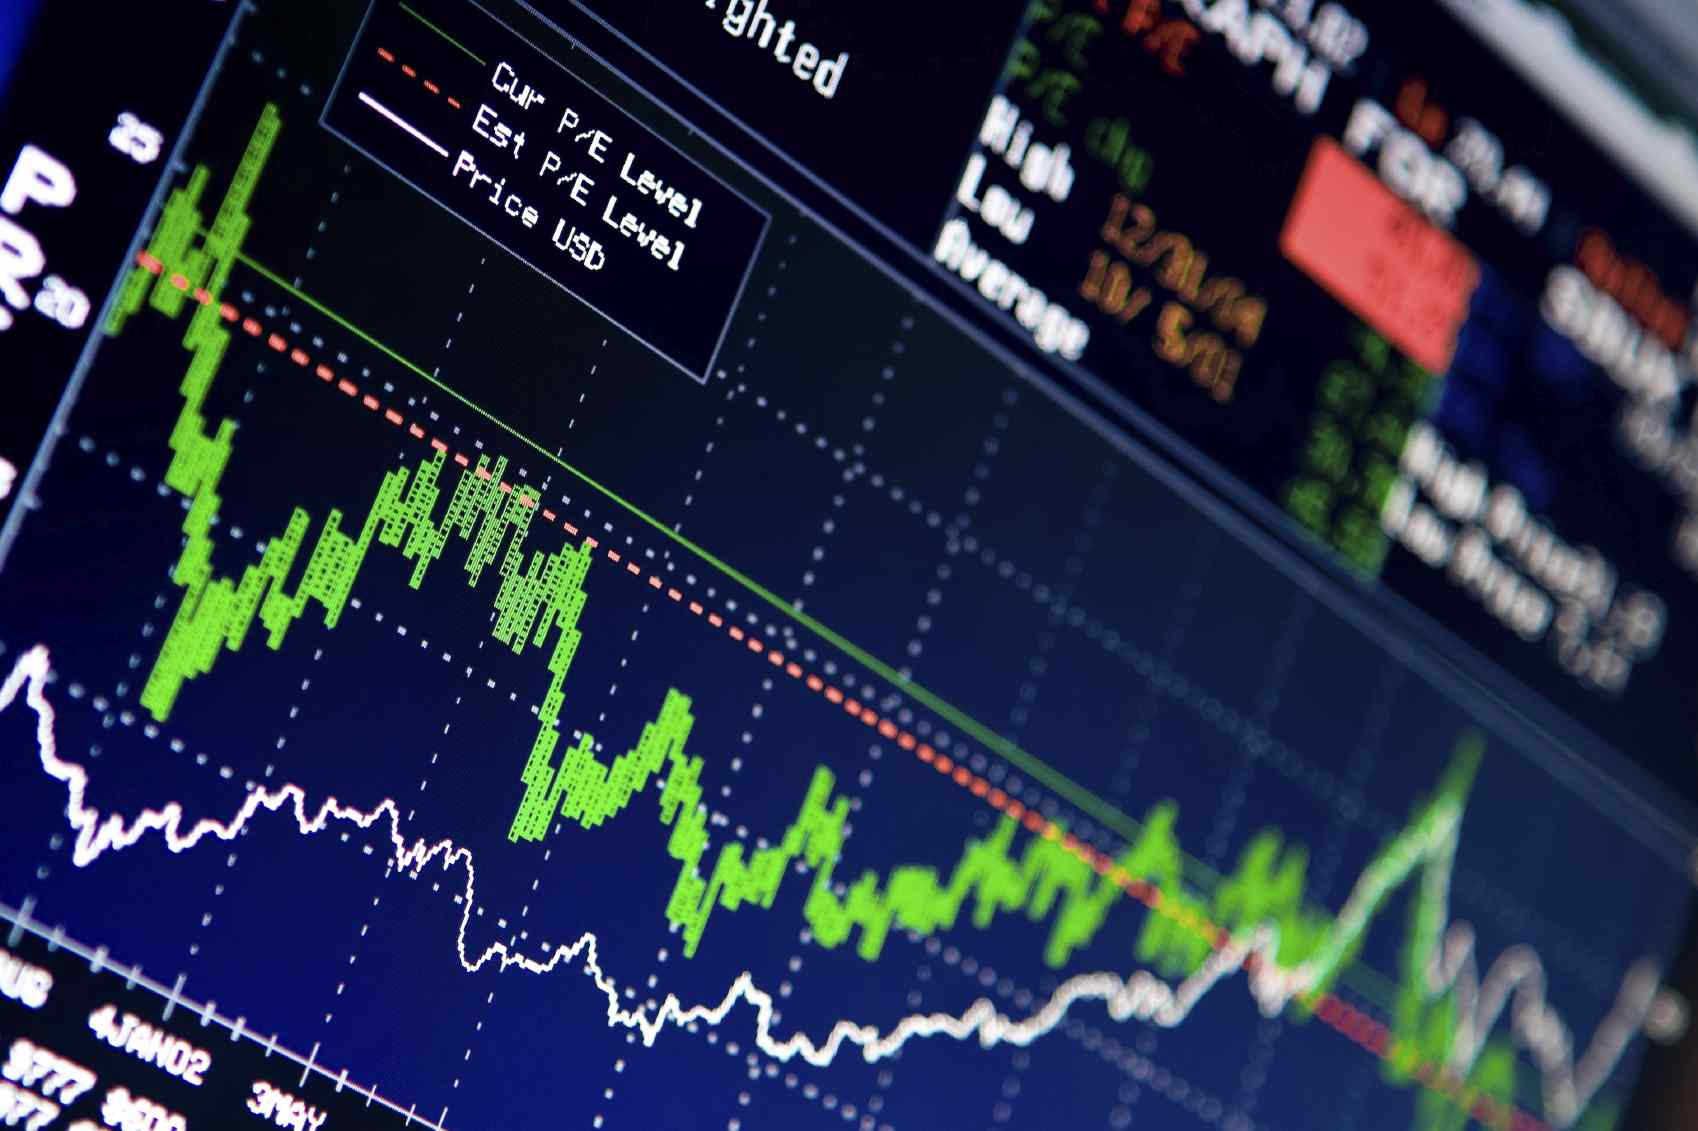
\includegraphics{stock-exchange}
}
%%% Title %%%%%%%%%%%%%%%%%%%%%%%%%%%%%%%%%%%%%%%%%%%%%%%%%%%%%%%%%%%%%%%%%%%%%
{\sf\bf
	Rankings of financial analysts \\as means to profits
}
%%% Authors %%%%%%%%%%%%%%%%%%%%%%%%%%%%%%%%%%%%%%%%%%%%%%%%%%%%%%%%%%%%%%%%%%%
{
	\vspace{1em} Artur Aiguzhinov, Carlos Soares, Ana Paula Serra\\
	{\smaller artur.aiguzhinov@inesctec.pt, csoares@fe.up.pt, aserra@fep.up.pt}
}
%%% Logo %%%%%%%%%%%%%%%%%%%%%%%%%%%%%%%%%%%%%%%%%%%%%%%%%%%%%%%%%%%%%%%%%%%%%%
{
% The logos are compressed a bit into a simple box to make them smaller on the result
% (Wasn't able to find any bigger of them.)
\setlength\fboxsep{0pt}
\setlength\fboxrule{0.5pt}
	\fbox{
		\begin{minipage}{18em}
			
\includegraphics[width=\linewidth]{INESC_TEC_04}
%			\includegraphics[width=4em,height=4em]{liaad-inesc} \\
%			\includegraphics[width=10em,height=4em]{liaad-inesc}
%			\includegraphics[width=4em,height=4em]{liaad-inesc}
		\end{minipage}
	}

}


\headerbox{Motivation}{name=problem,column=0,row=0}
{
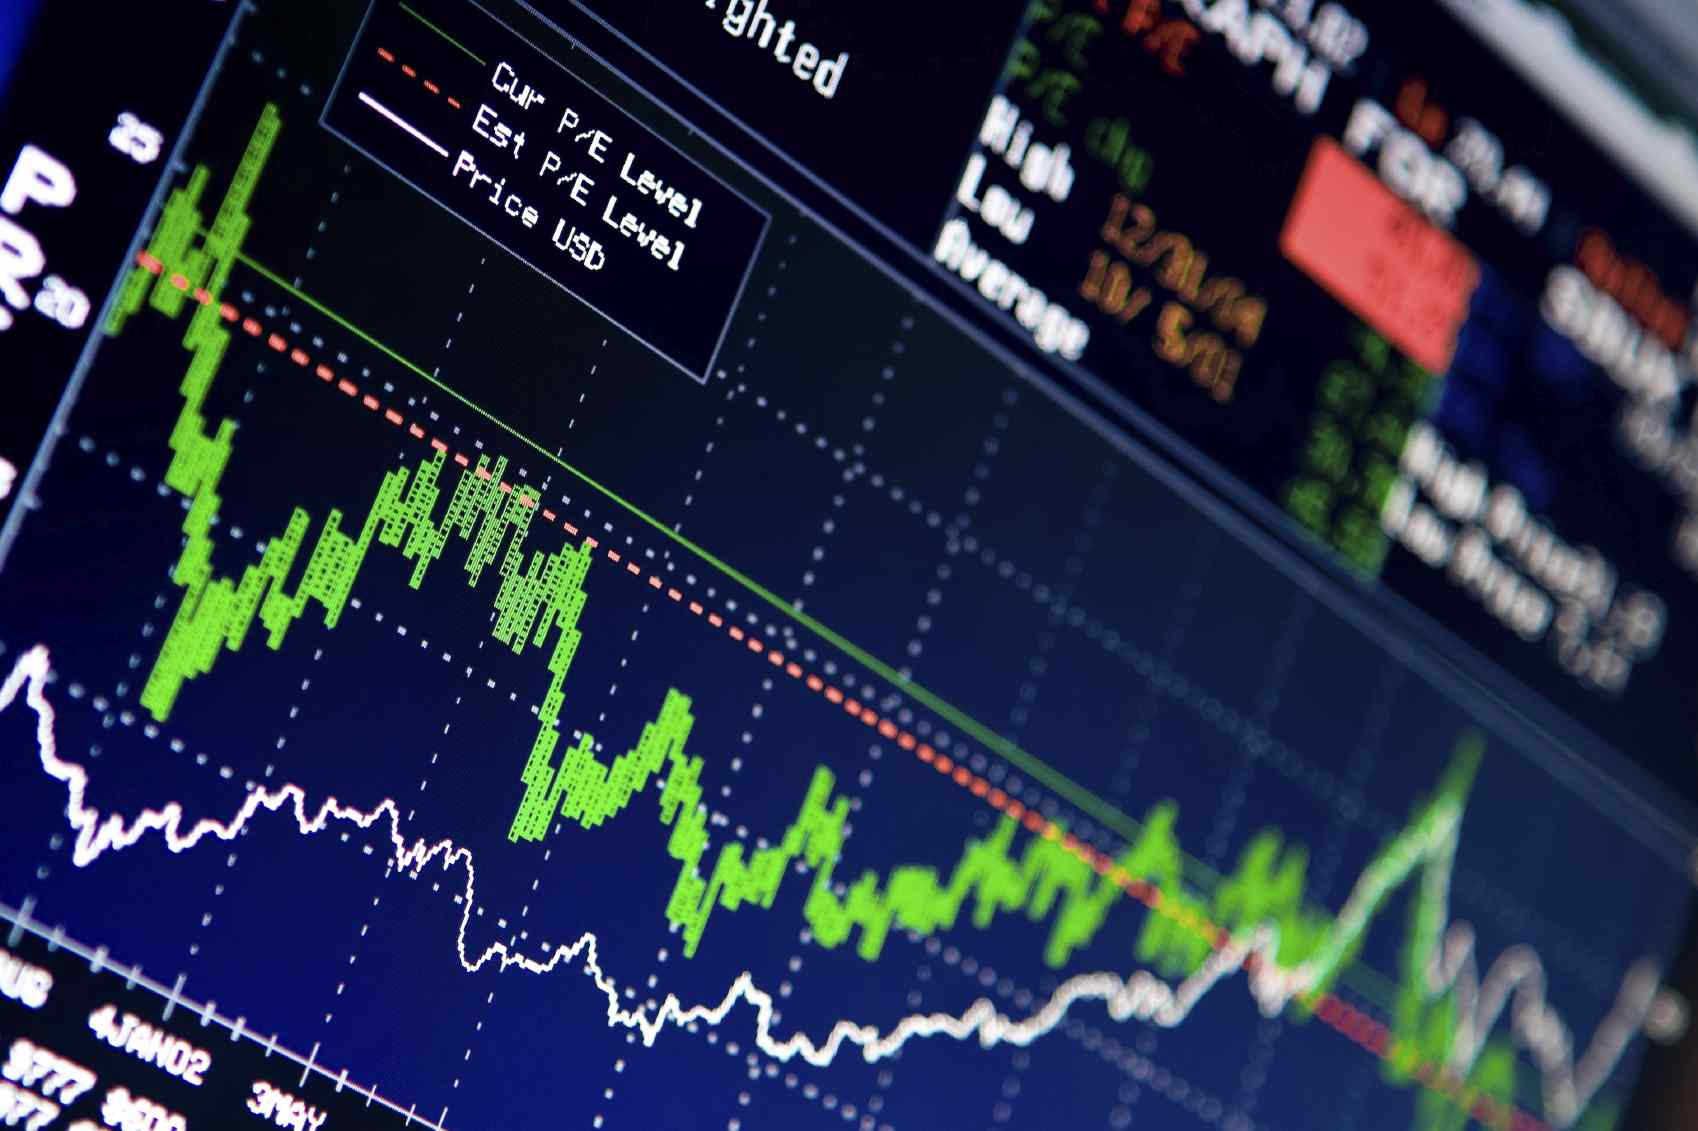
\includegraphics[ width=\linewidth]{stock-exchange}

\textbf{Rankings of financial analysts}:
\bi
\compresslist
\item Long debate on whether analysts create value to investors;
\item Rankings could be useful because they signal the top analysts.
\item Predicting the rankings of analysts can lead to  successful trading strategy based upon that information
\ei
}


\headerbox{Goal}{name=goal,column=0,below=problem}
{
\bi
\compresslist
\item Accurately predict the ranking of financial analysts
\item Develop a trading strategy based on predicted rankings
\ei
}


%
% \headerbox{Target Ranking}{name=tr,column=1,row=0}
% {
% Based on previous research, we use absolute error of earnings per share (EPS) forecasts as a measure of analysts' forecasting accuracy:
% $$
% \mathrm{FE_{q,a,s}}=|\mathrm{ActEPS_{q,s}}-\mathrm{EPS_{q,a,s}}|
% $$
% }

\headerbox{Label Ranking}{name=lr,span=1,column=0,below=goal}
{
\bi
\compresslist
\item  Instance: $\mathcal{X} \subseteq \{\mathcal{V}_1,\ldots,\mathcal{V}_m\}$
\item  Labels: $\mathcal{L} = \{\lambda_1,\ldots,\lambda_k\}$
 \item Output: $\mathcal{Y} = \Pi_{\mathcal{L}}$
 \item Training set: $\mathcal{T}=\{x_i,y_i\}_{i \in \{1, \ldots, n\}} \subseteq \mathcal{X} \times \mathcal{Y}$
 \ei
Learn a mapping $h: \mathcal{X} \rightarrow \mathcal{Y}$ such that a loss function $\ell$ is minimized:
\begin{equation}
\label{loss}
 \ell=\frac{\sum_{i=1}^n \rho(y_i,\hat{y}_i)}{n}
\end{equation}
with $\rho$ being a Spearman correlation coefficient:
\begin{equation}
\label{eq00}
 \rho(y,\hat{y})=1-\frac{6\sum_{j=1}^k(y_j-\hat{y}_j)^2}{k^3-k}
\end{equation}
where $y$ and $\hat{y}$ are, respectively, the target and predicted rankings for a given instance.

%' \small\addtolength{\tabcolsep}{-4pt}
%'
%'  \begin{tabular}{cccccccc}
%' \toprule
%' Period & $\mathcal{V}_1$ & $\mathcal{V}_2$ & $\mathcal{V}_3$ & $\mathcal{V}_4$ &\multicolumn{3}{c}{Ranks}\\
%' \cline{6-8}
%' &&&&&Alex&Brown&Credit\\
%' \midrule
%' <<echo=FALSE,results='asis'>>=
%' library(xtable)
%' data <- read.csv("~/Dropbox/workspace/Naive.Bayes.separate.functions/cont.data.csv", header = T, sep=",")
%'
%' ex.x <- matrix('x',nrow = 7,4)
%' for (i in seq_len(nrow(ex.x)))
%' {
%'   for (j in seq_len(ncol(ex.x)))
%'   {
%'     ex.x[i,j] <- paste0('$x_{',i,',',j,'}$')
%'   }
%' }
%'
%' print(xtable(cbind(data[1:7,1],ex.x,data[1:7,6:8])),only.contents=T,include.colnames=FALSE,include.rownames=F,hline.after=NULL, format.args=list(big.mark = " ", decimal.mark = "."),sanitize.text.function = function(x) x)
%' @
%' \bottomrule
%'  \end{tabular}
 }

\headerbox{Naive Bayes for LR}{name=nbr,column=1,row=0,span=1}
{
\small\addtolength{\tabcolsep}{-4pt}

Adapting naive Bayes classification algorithm requires defining posterior and conditional label ranking probabilities.  Define $\mathcal{S}$ as a similarity matrix between the target rankings in a training set, i.e. $\mathcal{S}_{n \times n}=\rho(y_i,y_j)$. The prior probability of a label ranking is given by:
\begin{equation}
P_{LR}(y) = \frac{\sum_{i=1}^{n} \rho(y,y_i)}{n}
\label{eq:prior}
\end{equation}

The conditional label ranking probability given its rankings is:
$$
P_{LR}(v_{a,i}|y)= \frac{\sum_{i: x_{i,a} = v_{a,i}}\rho(y, y_i)}{|\{i: x_{i,a} = v_{a,i}\}|}
$$
Extensions:
\bi
\compresslist
\item Case of continuous independent variables:
$$\label{cont}
P_{LR}(x_{i}|y)=\frac{1}{\sqrt{2\pi}\sigma_y}e^\frac{(x_i-\mu_y)^2}{2\sigma_y^2}
$$
where $\mu_y$ and $\sigma_y^2$ are weighted  mean and weighted variance and defined as follows:

$$\label{mu}
\mu_y =\frac{\sum_{i=1}^n  \rho(y,y_i) x_i}{\sum_{i=1}^n \rho(y,y_i)}
$$
$$\label{sigma}
\sigma_y^2=\frac{\sum_{i=1}^n \rho(y,y_i) (x_i-\mu_y)^2}{\sum_{i=1}^n \rho(y,y_i)}
$$

\item Timing in rankings:
$$P_{LR}(y) = \mathbf{w} \frac{\sum_{i=1}^{n} \rho(y,y_i)}{n}
\label{eq:timing}
$$
where $\mathbf{w}$ is the vector of weights calculated as:

$$\mathbf{w}=\alpha ^{\frac{T_{1 \ldots t}}{T}-1}  \;  \text{where} \; t \leqq T
$$
\ei
}

\headerbox{Trading strategy}{name=strategy,column=1,below=nbr}
{
The views are made of: $Q$---the expected stock return; $\Omega$---the confidence of $Q$. The trading strategy is applied as follows:
\begin{enumerate}
\compresslist
\item For each stock $s$, at the beginning of quarter $q$, we predict the rankings of all analysts that we expect to be at the end of the quarter $q$;
\item Based on these  predicted rankings and analysts' price targets,  we define $Q_{q,s}$ and $\Omega_{q,s}$;
\item Using market information available at the last day of quarter $q-1$, we obtain the market inputs;
\item Apply BL model to get  optimized portfolio weights and buy/sell stocks accordingly;
\end{enumerate}
}

\headerbox{Independent variables}{name=vvs,column=2,row=0}
{
State variables:
\bi
\compresslist
\item Analysts' dispersion;
\item Analysts' information asymmetry;
\item Analysts' uncertainty;
\item Stock return volatility;
\item Book-to-market ratio;
\item Debt-to-equity ratio;
\item Accruals;
\item Sector index volatility;
\item Interest rate;
\item Gross National Product;
\item Inflation rate;
\item Market volatility;
\ei

Methods of dynamics of the state variable:
\begin{itemize}
\compresslist
\item \raw{}---no dynamics of $x$;
\item  \diff{}---first-difference  of $x$;
\item  \random{}---an unobserved component of time series decomposition of $x$;
\item  \rollsd{}---moving 8 quarters standard deviation of $x$;
\end{itemize}
}

\headerbox{Data and experimental setup}{name=setup,column=2,below=vvs}
{
Databases:
\begin{itemize}
\compresslist
\item Analysts' Price targets data from ThomsonOne I/B/E/S Detailed History;
\item Stocks data from ThomsonOne DataStream:
\end{itemize}
Target rankings:
Given a  price target $\xi$, we, first define the  forecast error  ($\Delta$) as an absolute value of the difference between actual price $\xi_s$ and the price target made by an analyst $k$ ($\hat{\xi}_{k,s}$):
\begin{equation}
\Delta_{t,k,s}=|\xi_{t,s}-\hat{\xi}_{t,k,s}|
\end{equation}
Then, we calculate the average error across analysts as:
\begin{equation}
\overline{\Delta}_{t,s}=\frac{1}{k}\sum_{k=1}^k \Delta_{t,k,s}
\end{equation}
Next, PMAFE is given as:
\begin{equation}
\tilde{\Delta}_{t,k,s}=\frac{\Delta_{t,k,s}}{\overline{\Delta}_{t,s}}
\end{equation}

Different information sets:

\bi
\compresslist
\item \naive{} uses only the  information about the analyst's performance in period $t-1$;
\item \default{} uses all the available  information for that particular analyst.
\item \tr{} assumes we anticipate perfectly the future analyst accuracy performance  that would only be available at the end of $t$
\ei
}
\headerbox{Figure}{name=fig,column=2,below=setup}
{
\begin{center}
\begin{knitrout}
\definecolor{shadecolor}{rgb}{0.969, 0.969, 0.969}\color{fgcolor}
\includegraphics[width=0.7\linewidth]{figure/unnamed-chunk-3-1} 

\end{knitrout}
\end{center}
}

\headerbox{Results}{name=results,column=0,below=lr,span=2}
{
\small\addtolength{\tabcolsep}{-4pt}
\begin{center}
\begin{tabular}{cccccc}
    \toprule
Strategy&Return (in \%)&Std. dev (in \%)&SR&Num. stock&Turnover \\\midrule \textit{Market} & -3.032 & 16.654 & -0.182 &  499 & 0.053 \\ 
  
    \midrule
 \true{} & 1.785 & 15.312 & 0.117 &  240 & 0.272 \\ 
  \naive{} & 0.634 & 15.444 & 0.041 &  240 & 0.251 \\ 
  \default{} & 0.587 & 15.325 & 0.038 &  240 & 0.238 \\ 
  \last{} & 0.513 & 15.478 & 0.033 &  240 & 0.262 \\ 
  \diff{} & 0.779 & 15.507 & 0.050 &  240 & 0.269 \\ 
  \random{} & 0.671 & 15.474 & 0.043 &  240 & 0.258 \\ 
  \rollsd{} & 0.634 & 15.464 & 0.041 &  240 & 0.264 \\ 
  
  \bottomrule
  \end{tabular}
  \end{center}
}
\headerbox{Conclusion}{name=conclusion,column=0,below=results,span=2}
{
In this paper we developed an algorithm that is able to predict the rankings based on state variables that characterize the information environment of the analysts. Further, we designed and operationalized a trading strategy based on the Black-Litterman model with rankings as inputs. We obtained positive successful results from trading that out-performs both the market and the baseline ranking prediction.
}





%\headerbox{References}{name=references,column=0,below=design,span=1}{
%\smaller													% Make the whole text smaller
%\vspace{-0.4em} 										% Save some space at the beginning
%\bibliographystyle{plain}							% Use plain style
%\bibliography{/Users/aiguzhinov/Documents/Dropbox/Documents/Bibliography/rank}
%}


\end{poster}
\end{document}
